\documentclass{standalone}
\usepackage[utf8]{inputenc}
\usepackage[T1]{fontenc}
\usepackage{graphicx}
\usepackage{amsmath}
\usepackage[american,siunitx]{circuitikz}
\usetikzlibrary{arrows,shapes,calc,positioning}

\newcommand*{\pRC}[2]{%
  \begin{scope}[xshift=#1, yshift=#2] 
    \draw (0,0) -- (0.3, 0) -- (0.3, 0.5) to[R, ] (1.7, 0.5) -- (1.7, 0) -- (2,0); 
    \draw (0.3, 0) to[, *-,] (0.3, -0.5) to [C, ] (1.7,-0.5) -- (1.7, 0); 
  \end{scope}
}
    
\begin{document}
\begin{circuitikz}
  \def\ladderend{12}
  \def\relayr{0.4}
  \ctikzset{bipoles/thickness=1, bipoles/capacitor/height=0.4}

  \node (ton) at (4, -1) {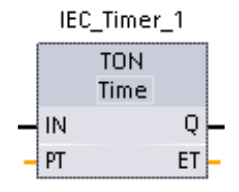
\includegraphics[width=2cm]{plc-TON.png}};
  \node[right of=ton, node distance=3cm] (tof) {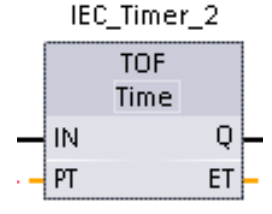
\includegraphics[width=2cm]{plc-TOF.png}};

  % Rail
  \draw[thick] (0,0) to[short,o-] (0,-3);
  \node[coordinate] (orig) at (0,0) {};      
  \node[coordinate] (tonin) at ($ (ton.west) + (0.3,-0.257) $) {};
  \node[coordinate] (tonout) at ($ (ton.east) + (-0.3,-0.257) $) {};
  \node[coordinate] (tofin) at ($ (tof.west) + (0.3,-0.248) $) {};
  \node[coordinate] (tofout) at ($ (tof.east) + (-0.3,-0.248) $) {};
  \node[coordinate, right of=tofout, node distance = 1cm] (coilin) {};
  \node[coordinate, right of=coilin, node distance = 1cm] (coilout) {};

  % Switch
  \draw[thick] (orig |- tonin) to[C={\%I0.0},] (tonin) (tonout) to[short] (tofin) 
     (tofout) to[short,] (coilin);
\end{circuitikz}
\end{document}
